\chapter{FPGA: historical introduction, structure, design flow, VHDL and use in the MoVe\_IT project}
\section{Introduction}
\noindent Digital electronics is concerned with circuits which represent information using a finite set of output
states. Most of the applications use in fact just two states, which are often labelled ‘0’ and ‘1’.
Behind this choice is the fact that the whole Boolean formalism then becomes available for the
solution of logic problems, and also that arithmetic using binary representations of numbers is a very
mature field\cite{fpga1}.
\newline
In addition, having only two
different values for the voltages or currents used to represent states is the safest choice in terms of
design margins in order to protect the data from the noise.



\section{Programmable Logic Devices history}
\noindent Historically, TTL (Transistor–Transistor Logic) chips fuelled an initial wave of digital system designs in
the 1970s.
%This section will focus on the separate branches that evolved to satisfy the demand
%for programmability of different logic functions.
By programmability, it is meant the ability of a
designer to affect the logic behaviour of a chip after it has been produced in the factory.
\newline
\noindent A first improvement in the direction of programmability came with the introduction of gate
arrays, which were nothing else than a chip filled with NAND gates that the designer could
interconnect as needed to generate any logic function he desired.
This interconnection had to happen
at the chip design stage, thus before production, but it was already a convenient improvement over
designing everything from scratch. Until the introduction of Programmable Logic
Arrays (PLAs) in the 1980s no real programmable solution was available. These were two-level AND-OR
structures with user-programmable connections.
%\begin{figure}[H]
%	\centering
%	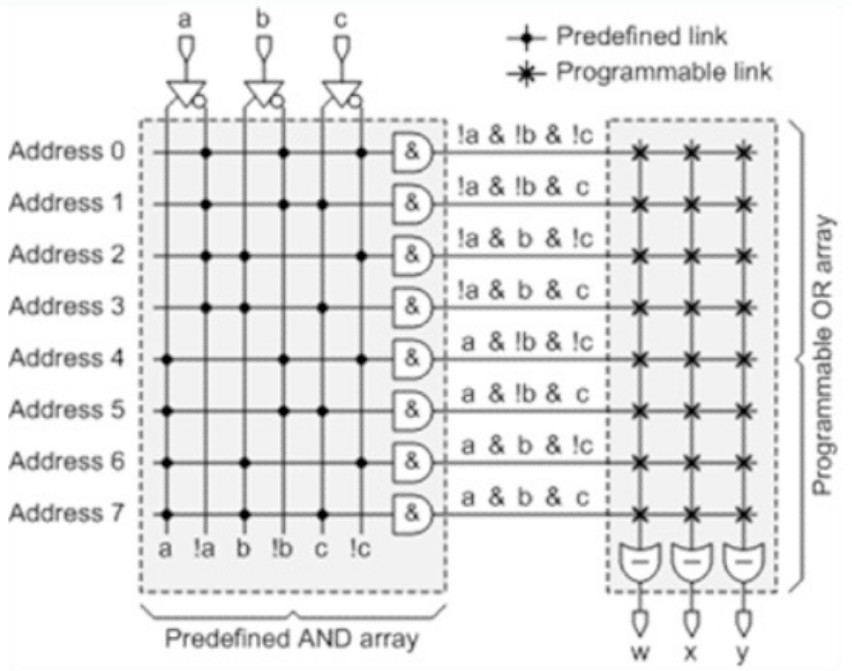
\includegraphics[width=0.7\linewidth]{IMG/ch3/PLD}
%	\caption{Unprogrammed PROM (Fixed AND Array, Programmable OR Array)}
%	\label{fig:pld}
%\end{figure}

\noindent Programmable Array Logic (PAL) devices were an
improvement in performance and cost over the PLA structure. Today, these devices are collectively
called Programmable Logic Devices (PLDs).

\noindent The next stage in sophistication resulted in Complex PLDs (CPLDs), which were nothing else
than a collection of multiple PLDs with programmable interconnections. FPGAs, in turn, contain a
much larger number of simpler blocks with the attendant increase in interconnect logic, which in fact
dominates the entire chip.
\begin{figure}[H]
	\centering
	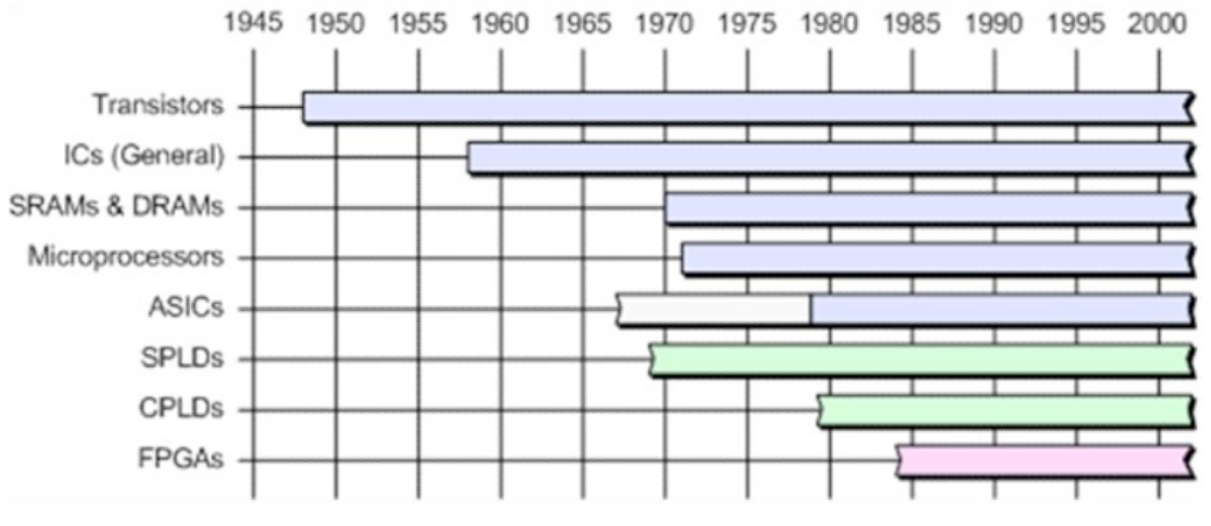
\includegraphics[width=0.7\linewidth]{IMG/ch3/TIME}
	\caption{Appearance over the years of programmable logic devices\cite{fpga3}}
	\label{fig:time}
\end{figure}
%\subsection{FPGA}
\noindent Xilinx introduced the first Field Programmable Gate Arrays
(FPGAs) in 1984, though they were not called FPGAs until
Actel popularized the term around 1988\cite{fpga2}. Since their introduction, FPGA devices have progressed
through several distinct phases of development.
Each phase was driven by both process technology opportunity
and application demand. These driving pressures
caused observable changes in the device characteristics
and tools. Each age is eight years long and each
became apparent only in retrospect. The three ages are:
\begin{itemize}
	\item Age of Invention 1984–1991
	\newline
	In the Age of Invention, FPGAs were small, so the design problem was small. Though they were desirable, synthesis
	and even automated placement and routing were not considered essential. Many deemed it impractical even to
	attempt design automation on the personal computers of the time, since ASIC placement and routing was being
	done on mainframe computers.
	Manual design, both
	logical and physical, was acceptable because of the small problem size. Manual design was often necessary because
	of the limited routing resources on the chips.
	Radically different architectures precluded universal FPGA design tools, as were available in the ASIC business.
	FPGA vendors took on the added burden of EDA (Electronic Design Automation) development for their devices and this was eventually recognized as an advantage.
	\newline
	In the Age of Invention, FPGAs were much smaller than the applications that users wanted to put into them. As a
	result multiple-FPGA systems became popular and automated multi-chip partitioning software was identified as
	an important component of an FPGA design suite, even as automatic placement and routing were not.
	\item Age of Expansion 1992–1999
	\newline
	Through the Age of Expansion, Moore’s Law rapidly increased the capacity of FPGAs, leading to a demand for
	design automation and permitting longer interconnect segmentation.
	FPGAs encroached on ASIC territory as FPGA device capacity grew more rapidly than the
	demand from applications. No longer did users clamor for multi-FPGA partitioning software.
	As FPGAs became more popular, EDA companies became interested in providing tools for them.
	\item Age of Accumulation 2000–2007
	\newline
	The biggest change in FPGAs in the Age of Accumulation was the change in the target application. The FPGA
	business grew not from general ASIC replacement, but from adoption by the communications infrastructure. Companies
	such as Cisco Systems used FPGAs to make custom data paths for steering huge volumes of internet and packetized
	voice traffic through their switches and routers.
	By the end of the 2000s, FPGAs were not general-purpose ASIC replacements as much as they were data-routing engines.
	FPGA bitwise programmability assured their continued use in a wide range of applications, including control and automotive systems.
\end{itemize}

\section{FPGA Versus PAL}
\noindent Programmable logic was well established before the
FPGA. EPROM-programmed Programmable Array Logic
(PAL) had carved out a market niche in the early 1980s.
However, FPGAs had an architectural advantage. To understand
the FPGA advantage, we first look at the simple
programmable logic structures of these early 1980s devices.
A PAL device, as depicted in figure \ref{fig:pal}, consists of a two level
logic structure. Inputs are shown entering at
the bottom. On the left side, a programmable and array
generates product terms, ands of any combination of the
inputs and their inverses. A fixed or gate in the block at
the right completes the combinational logic function of the
macrocell’s product terms. Every macrocell output is an
output of the chip.
\begin{figure}[H]
	\centering
	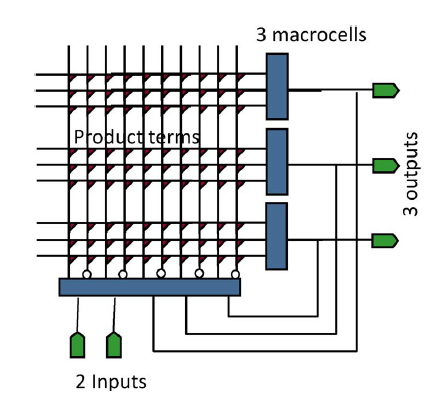
\includegraphics[width=0.7\linewidth]{IMG/ch3/PAL}
	\caption{Generic PAL architecture}
	\label{fig:pal}
\end{figure}
\noindent Nearly all common functions could be implemented in one pass through the PAL's macrocell array.
The delay through the PAL array is the same regardless of the function performed or where it is located in the array.
PALs had simple fitting software that mapped logic quickly to arbitrary locations in the array with no performance concerns.
PALs were very efficient from a manufacturing point of view.
However, the architectural issue with PALs is evident when one considers scaling. The number of programmable points in
the and array grows with the square of the number of inputs. PAL input and product-term lines are also
heavily loaded, so delay grows rapidly as size increases. To maintain speed, power consumption rose dramatically. Large PALs were
impractical in both area and performance.
\newline
The FPGA innovation was the elimination of the and array that provided the programmability. Instead, configuration
memory cells were distributed around the array to control functionality and wiring. This change gave up the
memory-array-like efficiency of the PAL structure in favor of architectural scalability. The architecture of the FPGA,
shown in figure 4, consists of an array of programmable logic blocks and interconnect with field-programmable switches.
\begin{figure}[H]
	\centering
	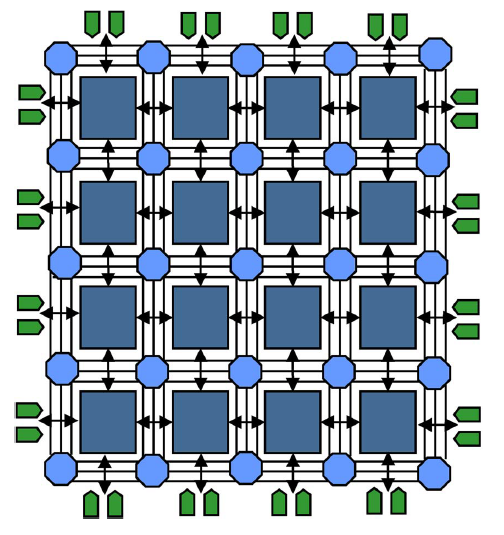
\includegraphics[width=0.7\linewidth]{IMG/ch3/FPGA}
	\caption{Generic array FPGA architecture. 4x4 array with three wiring
		tracks per row and column. Switches are at the circles at intersections.
		Device inputs and outputs are distributed around the array.}
	\label{fig:fpga}
\end{figure}
\noindent The consequences of this change were:
\begin{itemize}
	\item FPGA architecture could look nothing like a memory. Design and manufacturing were very different than memory.
	\item The logic blocks were smaller. There was no guarantee that a single function would fit into one. Therefore, it was difficult to determine ahead of time how much logic would fit into the FPGA.
	\item The performance of the FPGA depended on where the logic was placed in the FPGA. FPGAs required placement and routing, so the performance of the finished design was not easy to predict in advance.
	\item Complex EDA software was required to fit a design into an FPGA.
\end{itemize}




\section{FPGA vs ASIC}
\noindent In the 1980s, Application-Specific Integrated Circuit
(ASIC) companies brought an amazing product to the
electronics market: the built-to-order custom integrated
circuit. By the mid-1980s, dozens of companies were selling
ASICs, and in the fierce competition, the winning attributes
were low cost, high capacity and high speed.When
FPGAs appeared, they compared poorly on all of these
measures, yet they thrived. The ASIC functionality was determined by custom mask
tooling. ASIC customers paid for those masks!
Because they had no custom tooling, FPGAs reduced the up-front
cost and risk of building custom digital logic. By making
one custom silicon device that could be used by hundreds or
thousands of customers, the FPGA vendor effectively
amortized the costs over all customers.
\begin{figure}[H]
	\centering
	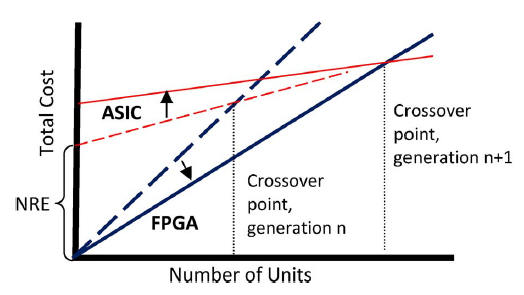
\includegraphics[width=0.7\linewidth]{IMG/ch3/COST}
	\caption{FPGA versus ASIC Crossover Point. Graph shows total cost
		versus number of units. FPGA lines are darker and start at the lower
		left corner. With the adoption of the next process node (arrows
		from the earlier node in dashed lines to later node in solid lines),
		the crossover point, indicated by the vertical dotted line, grew larger.
	\newline NRE (non-recurring engineering cost).}
	\label{fig:cost}
\end{figure}     
\noindent  An FPGA has no NRE charge, but each unit costs more than the
functionally equivalent ASIC, hence the steeper line. The
two lines meet at the crossover point. If fewer than that
number of units is required, the FPGA solution is cheaper;
more than that number of units indicates the ASIC has
lower overall cost.
\newline
Today, device cost is less of a driver in the FPGA
versus ASIC decision than performance, time-to-market,
power consumption, I/O capacity and other capabilities. Many ASIC customers use older process technology,
lowering their NRE cost, but reducing the per-chip cost
advantage. Not only did FPGAs eliminate the up-front masking
charges and reduce inventory costs, but they also reduced
design costs by eliminating whole classes of design problems.
These design problems included transistor-level design,
testing, signal integrity, crosstalk, I/O design and
clock distribution.

\section{FPGA structure}
\begin{figure}[H]
	\centering
	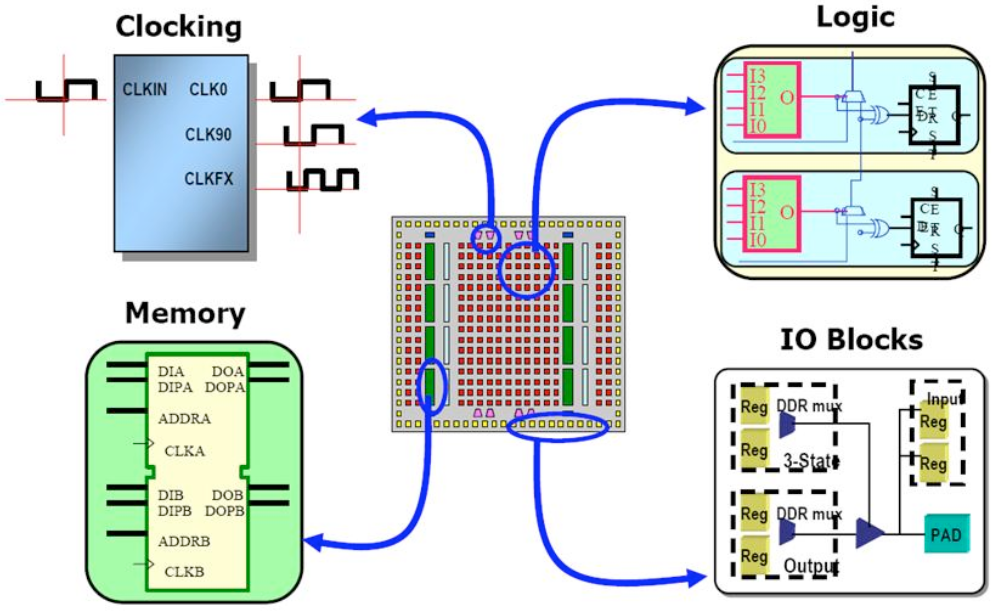
\includegraphics[width=0.7\linewidth]{IMG/ch3/FPGA2}
	\caption{Internal structure of a generic FPGA}
	\label{fig:fpga2}
\end{figure}
\noindent A typical modern FPGA, like in figure \ref{fig:fpga2}, provides the user with programmable logic blocks that
contain the pool of combinatorial blocks and flip-flops to be used in the design. In addition, vendors
acknowledge the fact that logic is often used with memory, and typically include
variable amounts of static Random Access Memory (RAM) inside their chips. Clock conditioning has
also become commonplace, and support in the form of Delay Locked Loops (DLLs) and Phase Locked
Loops (PLLs) is also provided inside the same silicon chip. Finally, an FPGA chip needs to be easily interfaced to other chips or
external signals. In order to make this interfacing easier, FPGA vendors have invested a great deal of
effort in enhancing the flexibility of the input/output blocks behind the chip pads. Each pad can serve
as an input, an output, or both. The list of electrical standards supported is extensive, and novel
techniques for maximizing bandwidth, such as clocking data in using both edges of the clock, are
widely supported.
\newline
All the components shown in figure \ref{fig:fpga2}, however, typically account for less than 20\% of the silicon
inside an FPGA chip. What is not shown is the large amounts of programmable interconnect and the
auxiliary circuits which ‘program’ the generic blocks to become a well-defined piece of logic.
To overcome the silicon inefficiency problem, FPGA vendors often include hardwired
Intellectual Property (IP) cores inside the chips for functions identified as recurrent in many designs.
These non-programmable blocks include general-purpose processors, high-speed serial interfaces,
arithmetic blocks and Ethernet Medium Access Control (MAC) units.
\\
FPGAs are truly parallel in nature so different processing operations do not have to compete for the same resources. As a result, the performance of one part of the application is not affected when additional processing is added.
\newline
\noindent In figure \ref{fig:fpga} it can be seen that the three more important blocks that made a FPGA chip are: Configurable logic Blocks (CBLs, blue squares); Input/Output Blocks (IOBs, green rectangles); Programmable Switch Matrixs (PSMs, blue octagon).
\begin{itemize}
	\item \textbf{CBLs}: Each CLB consists of n-input Lookup table and a pair of programmable flip flops. In Xilinx logic block, figure \ref{fig:clb}, a Look up table is used to implement any number of different functionality. The output of the lookup table gives the result of the logic function that it implements. Lookup table is implemented using SRAM (Static Random Access Memory).
	\begin{figure}[H]
		\centering
		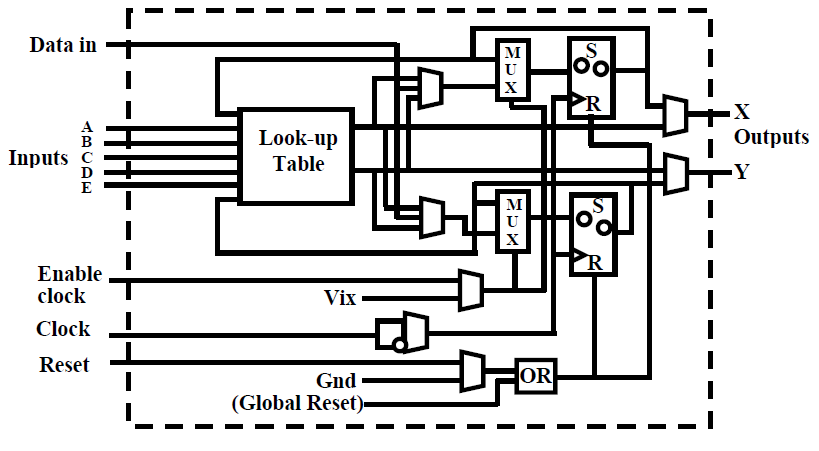
\includegraphics[width=0.7\linewidth]{IMG/ch3/CLB}
		\caption{Xilinx - LUT based configurable logic block}
		\label{fig:clb}
	\end{figure}
	\item \textbf{IOBs}: I/O blocks control functions such as tri-state buffer control, output transition speed (Slew Rate).
	\newline
	Provides to the chip a minimum of over-current and over-voltage protection and the right termination for each specific type of signalling.
	\item \textbf{PSMs}: Interconnects provide routing path. Using 6 CMOS switches controlled by a 6-bit data can be controlled a  wire intersection. Being \textbf{A}, \textbf{B}, \textbf{C} and \textbf{D} the  end of the routing the following connections can be made: \textbf{AB}, \textbf{AC}, \textbf{AD}, \textbf{BC}, \textbf{BD} and \textbf{CD}.
	\newline
	The data for each PSM is stored in a SRAM.
\end{itemize}
\noindent Thus a board its configured in two ways:
\begin{itemize}
	\item By setting the intersections (SMBs) between the logic blocks.
	\item By setting the function of each logic block.
\end{itemize}
\section{FPGA design flow and tools}
\noindent The most common flow nowadays used in the design of FPGAs involves the following
subsequent phases:
\begin{itemize}
	\item \textbf{Design entry}: This step consists in transforming the design ideas into some form of
	computerized representation. This is most commonly accomplished using Hardware Description
	Languages (HDLs). The two most popular HDLs are Verilog and the Very High Speed
	Integrated Circuit HDL (VHDL), used fot my thesis work. It should be noted that an HDL, as its name implies, is only
	a tool to describe a design that pre-existed in the mind, notes, and sketches of a designer. Another point to note is that HDLs differ from
	conventional software programming languages in the sense that they don’t support the concept
	of sequential execution of statements in the code. This is easy to understand if one considers the
	alternative schematic representation of an HDL file: what one sees in the upper part of the
	schematic cannot be said to happen before or after what one sees in the lower part.
	This is the only human-labour intensive part of the design process.
	\item \textbf{Simulation}: Typically, the design entry step is followed or interspersed with periods of functional simulation. That's where a simulator is used to execute the design and confirm that the correct outputs are produced for a given set of test inputs\cite{fpga4}. This section will be analyzed in more detail later on in this chapter.
	\item \textbf{Synthesis}: The synthesis tool receives HDL and a choice of FPGA vendor and model. From
	these two pieces of information, it generates a netlist which uses the primitives proposed by the
	vendor in order to satisfy the logic behaviour specified in the HDL files.
	\item \textbf{Place and route}: The placer takes the synthesized netlist and chooses a place for each of the
	primitives inside the chip. The router’s task is then to interconnect all these primitives together
	satisfying the timing constraints. The most obvious constraint for a design is the frequency of
	the system clock, but there are more involved constraints one can impose on a design using the
	software packages supported by the vendors.
	\item \textbf{Bit stream generation (Download)}: FPGAs are typically configured at power-up time from some sort of
	external permanent storage device, typically a flash memory. Once the place and route process is
	finished, the resulting choices for the configuration of each programmable element in the FPGA
	chip, be it logic or interconnect, must be stored in a file to program the flash.
	
\end{itemize}

\begin{figure}[H]
	\centering
	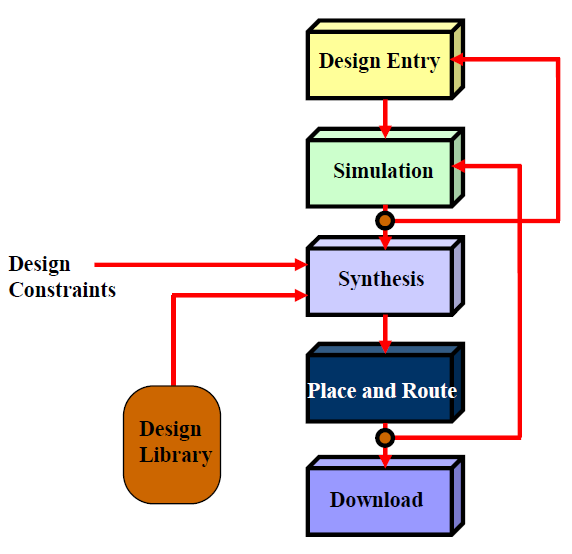
\includegraphics[width=0.6\linewidth]{IMG/ch3/FLOW}
	\caption{Programmable logic, in this case FPGA, design process}
	\label{fig:flow}
\end{figure}

\section{Hardware Description Language}
\noindent Hardware description language (HDL) is a specialized computer language used to describe the structure and behaviour of electronic circuits, and most commonly, digital logic circuits\cite{hdl}. A hardware description language looks like a programming language similar to C; it is a textual description consisting of expressions, statements and control structures. One important difference between most programming languages and HDLs is that HDLs explicitly include the notion of time.
HDLs form an integral part of EDA systems, especially for complex circuits, such as ASICs, PLDs and FPGAs.
\newline
The first hardware description languages appeared in the late 1960s, looking like more traditional languages.
By the late 1970s, design using PLDs became popular, although these designs were primarily limited to designing finite-state machines.
In 1985 Gateway Design Automation introduced Verilog and Intermetrics released the first completed version of the VHSIC (Very High Speed Integrated Circuit) Hardware Description Language (VHDL).
VHDL was developed at the behest of the United States Department of Defence's VHSIC program.
Within a few years, VHDL and Verilog emerged as the dominant HDLs in the electronics industry.
\subsection{VHDL}
\noindent The biggest part of the FPGA firmware used in the MoVe\_IT project is written in VHDL\cite{vhdl}. This HDL was invented to describe hardware and in fact VHDL is a concurrent language. What this means is that, normally, VHDL instructions are all executed at the same time (concurrently), regardless of the size of the needed implementation. Thus the VHDL model can be translated into a form that can be used to generate actual working circuits.
\begin{figure}[H]
	\centering
	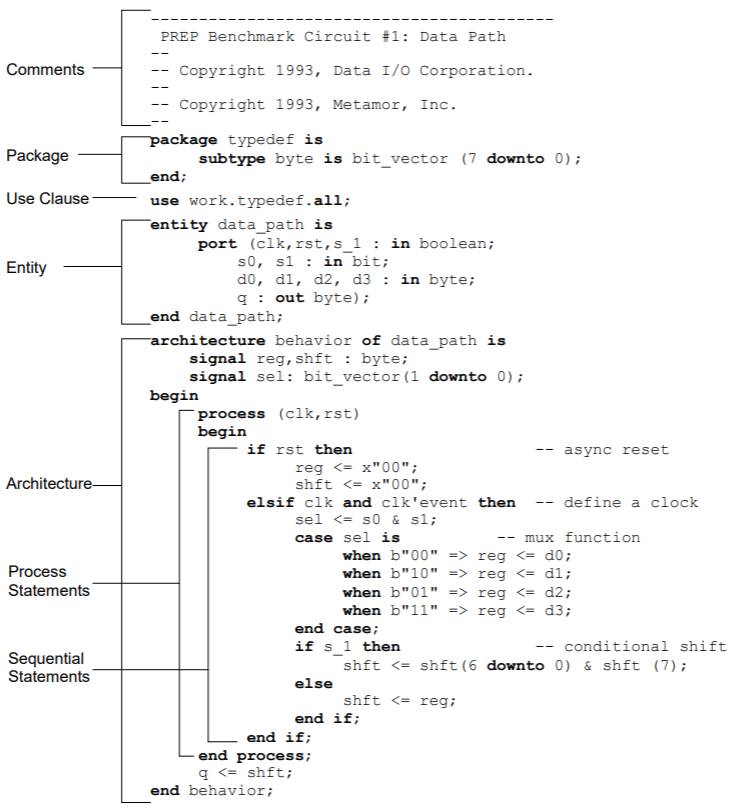
\includegraphics[width=0.7\linewidth]{IMG/ch3/VHDL}
	\caption{The structure of a VHDL design description}
	\label{fig:vhdl}
\end{figure}

\subsection{Entity}
\noindent A digital system is structured as a hierarchic collection of modules. Each module, that can be  has a series of ports that enables him to communicate with the external world. The VHDL entity provides a simple wrapper for the
lower-level circuitry. This wrapper effectively describes how the black box interfaces with the outside world. Since VHDL describes digital circuits, the entity simply lists the various inputs and outputs of the underlying circuitry.
\begin{figure}
	\centering
	\begin{minipage}{.5\textwidth}
		\centering
		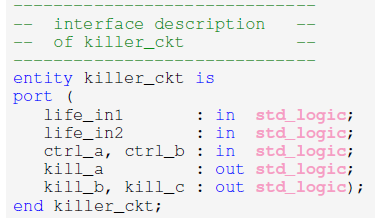
\includegraphics[width=.7\linewidth]{IMG/ch3/ENTITY2}
		\caption{VHDL entity declaration}
		\label{fig:entity2}
	\end{minipage}%
	\begin{minipage}{.5\textwidth}
		\centering
		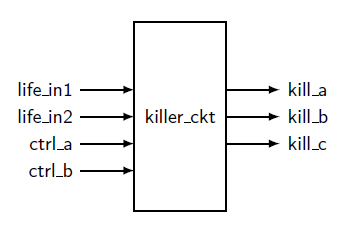
\includegraphics[width=.62\linewidth]{IMG/ch3/ENTITY1}
		\caption{Black box design example}
		\label{fig:entity1}
	\end{minipage}
\end{figure}
\noindent In figure \ref{fig:entity2} it can be seen that each port matches an arrow in figure \ref{fig:entity1}; the arrow goes inside the black box for an input and outside for an output. The data type std\_logic is what the IEEE has standardized for the representation of digital signals. 

\subsection{Architecture}
\noindent The VHDL entity declaration, introduced before, describes the interface or the external representation of the circuit. The architecture describes what the circuit actually does.
There can be any number of equivalent architectures describing a single entity. The VHDL coding style used inside
the architecture body has a significant effect on the way the circuit is
synthesized, thus how the circuit will be implemented inside an actual silicon device.
An architecture can be written by means of three modelling techniques
plus any combination of these three. There is the data-flow model, the behavioural model and the structural model.
\begin{itemize}
	\item \textbf{data-flow model}:
	\newline
	In the data-flow approach, circuits are described by showing the input and output relationships between the various built-in components of the VHDL language. The built-in components of VHDL include operators such as AND, OR, XOR, etc.
	It is good that it can be seen the flow of data in the circuit by examining the VHDL code, however data-flow modelling works fine for small and relatively simple circuits; as circuits become more complicated, it is often advantageous
	to switch to behavioural style models.
	\item \textbf{behavioural model}:
	\newline
	The behavioural style architecture provides no details as to how the design is implemented in actual hardware.
	Instead, the behavioural style models how the circuit outputs will react to the circuit inputs.
	Behavioural modelling is considered higher up on the circuit abstraction level as compared to data-flow models. It is the
	VHDL synthesizer tool that decides the actual circuit implementation.
	The heart of the behavioural style architecture is the process statement.
	\item \textbf{structural model}:
	\newline
	As digital designs become more complex, it becomes less likely that any one design can be implemented with any one of the three types of VHDL models. Most complex designs could be considered structural models. Modular designs promote understandability by packing low-level functionality into modules.
	The VHDL structural model supports the reuse of design units. This includes units that have been previously designed as well as the ability to use predefined module libraries.
	
\end{itemize}

\subsection{Process}
\noindent The process statement is a statement which contains a certain number of instructions that, when the process statement is executed, are executed sequentially. In other words, the process statement is a tool that can be used any time it is needed to execute a certain number of instructions in a sequential manner, one instruction after the other, from top to bottom.
\newline
The process statement in itself is a concurrent statement and therefore will be executed together with the other concurrent statements in the body of the architecture where it sits, like in figure \ref{fig:vhdl}.

\subsection{Constraints}
\noindent Constraints\cite{constraints1} are used to influence the FPGA design implementation tools including the
synthesizer, and place-and-route tools. They allow the user to specify the design
performance requirements and guide the tools toward meeting those requirements. The
implementation tools prioritize their actions based on the optimization levels of synthesis,
specified timing, assignment of pins, and grouping of logic provided to the tools by the user.
There are two main type of constraints: 
\begin{itemize}
	\item \textbf{Logical constraints} are constraints that are attached to elements in the design prior to
	mapping or fitting. Applying logical constraints helps to adapt the design performance to expected worst-case conditions. Later, when choosing a specific Xilinx architecture and place and route or fit the design, the logical constraints are converted into physical constraints\cite{constraints2}.
	\newline
	There are three main categories of logical constraints:
	\begin{itemize}
		\item Placement constraints
		\item Relative Location (RLOC) constraints
		\item Timing constraints
	\end{itemize}
	Timing constraints allow to specify the maximum allowable delay or skew on any given set of paths or nets in the design.
	
	\item \textbf{Physical constraints}. Constraints can also be attached to the elements in the physical design, that is, the design
	after mapping has been performed. These constraints, like I/O pin selection, are referred to as physical constraints.	 
\end{itemize}
\noindent XDC constraints are a combination of industry standard Synopsys Design Constraints (SDC) and Xilinx proprietary physical constraints. XDC constraints have the following properties:
\begin{itemize}
	\item They are not simple strings, but are commands that follow the Tcl (Tool command language) semantic.
	\item They can be interpreted like any other Tcl command by the Vivado Tcl interpreter.
	\item They can be stored in one or more XDC files.
\end{itemize}

\section{Development tools}

\subsection{Vivado}
\noindent In the MoVe\_IT project for the simulation, synthesis and implementation of the firmware it was used only Xilinx Vivado software.
\newline
Vivado Design Suite is a software suite produced by Xilinx for synthesis and analysis of HDL designs. It has also its own text editor, however it is not the most efficient tool for writing code.
Vivado includes a in-built logic simulator, high-level synthesis, an IP (Intellectual Property) Integrator, and a toolchain that converts C code into programmable logic\cite{vivado}.
This tool supports both VHDL and Verilog and can manage mixed language projects.
For this project was used the Vivado 2015.4 version. 
\begin{figure}[H]
	\centering
	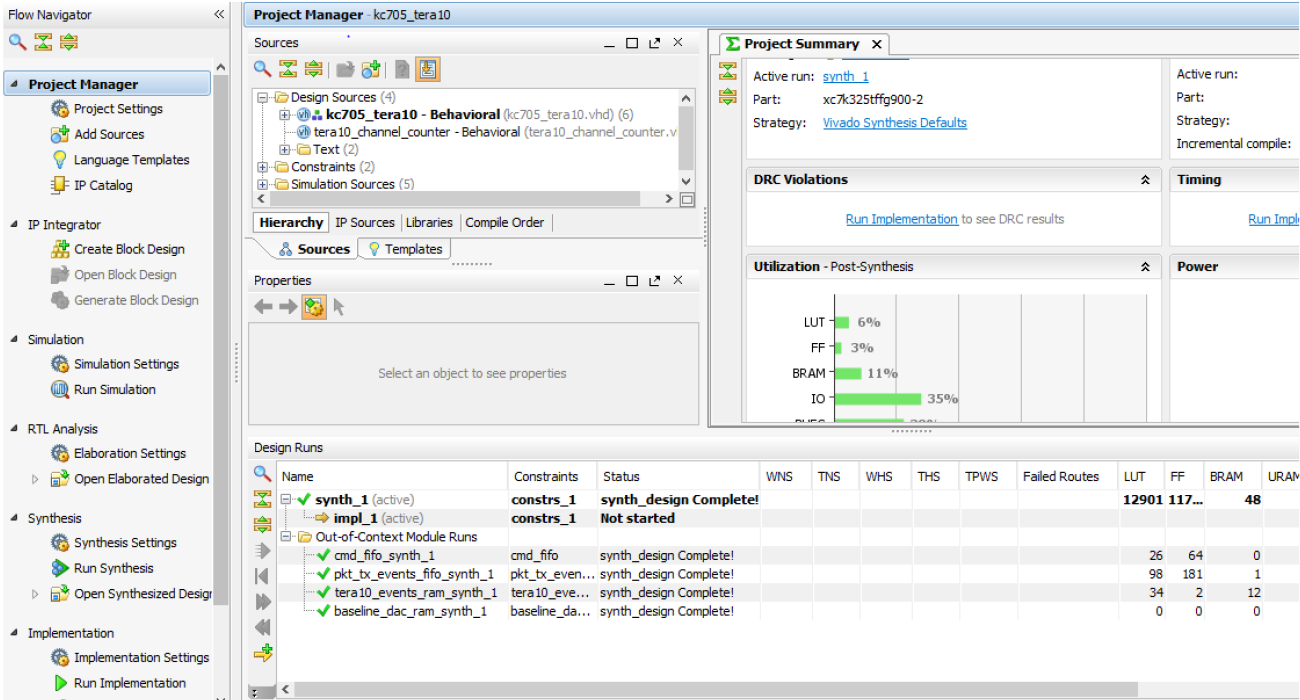
\includegraphics[width=0.9\linewidth]{IMG/ch3/VIVADO}
	\caption{Vivado 2015.4 project mode working environment}
	\label{fig:vivado}
\end{figure}

\subsection{LabVIEW}
\noindent Laboratory Virtual Instrument Engineering Workbench (LabVIEW) is a system-design platform and development environment for a visual programming language from National Instruments. The graphical language is named "G". LabVIEW is commonly used for data acquisition, instrument control, and industrial automation on a variety of operating systems.
LabVIEW integrates the creation of user interfaces (termed front panels) into the development cycle. LabVIEW programs-subroutines are termed virtual instruments (VIs). Each VI has three components: a block diagram, a front panel, and a connector pane.
The front panel is built using controls and indicators. Controls are inputs: they allow a user to supply information to the VI. Indicators are outputs: they indicate, or display, the results based on the inputs given to the VI. The back panel, which is a block diagram, contains the graphical source code.
\begin{figure}[H]
	\centering
	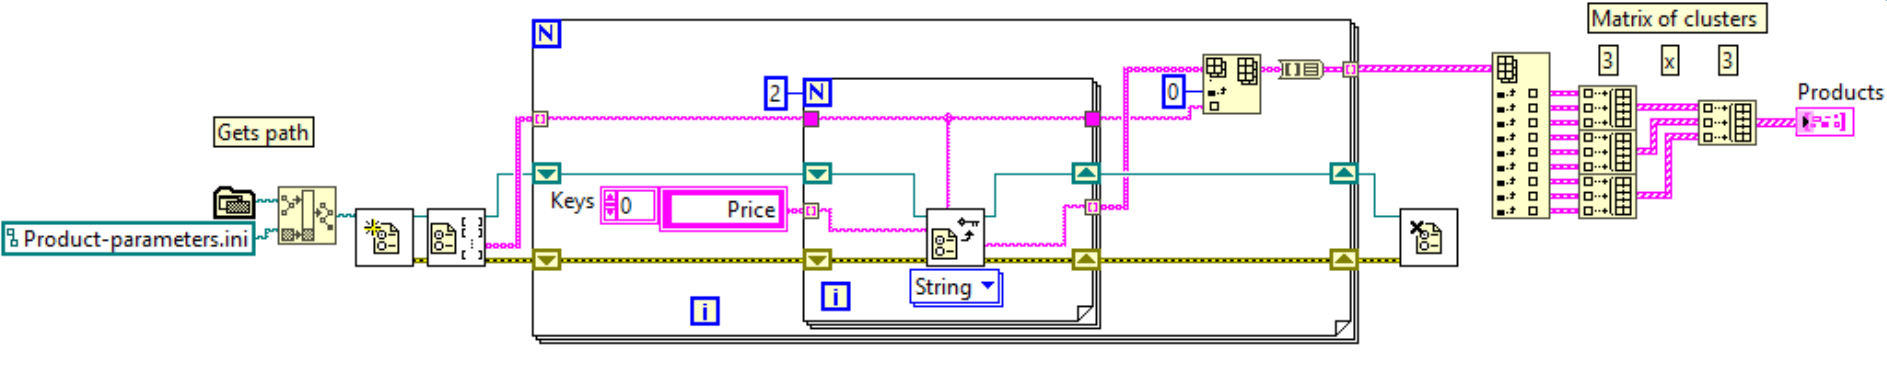
\includegraphics[width=0.9\linewidth]{IMG/ch3/LABVIEW}
	\caption{LabVIEW example project}
	\label{fig:labview}
\end{figure}
\noindent The graphical approach also allows "non-programmers" to build programs by dragging and dropping virtual representations of lab equipment with which they are already familiar.
\newline
LabVIEW includes extensive support for interfacing to devices such as instruments, cameras, and other devices like, in this case, FPGA boards.
\newline
In figure \ref{fig:labview2} it can be seen the LabVIEW program that controls (writes and reads) the internals DACs for the ABACUS2 chip; it will be analyzed more in depth in the next chapter.
\begin{figure}[H]
	\centering
	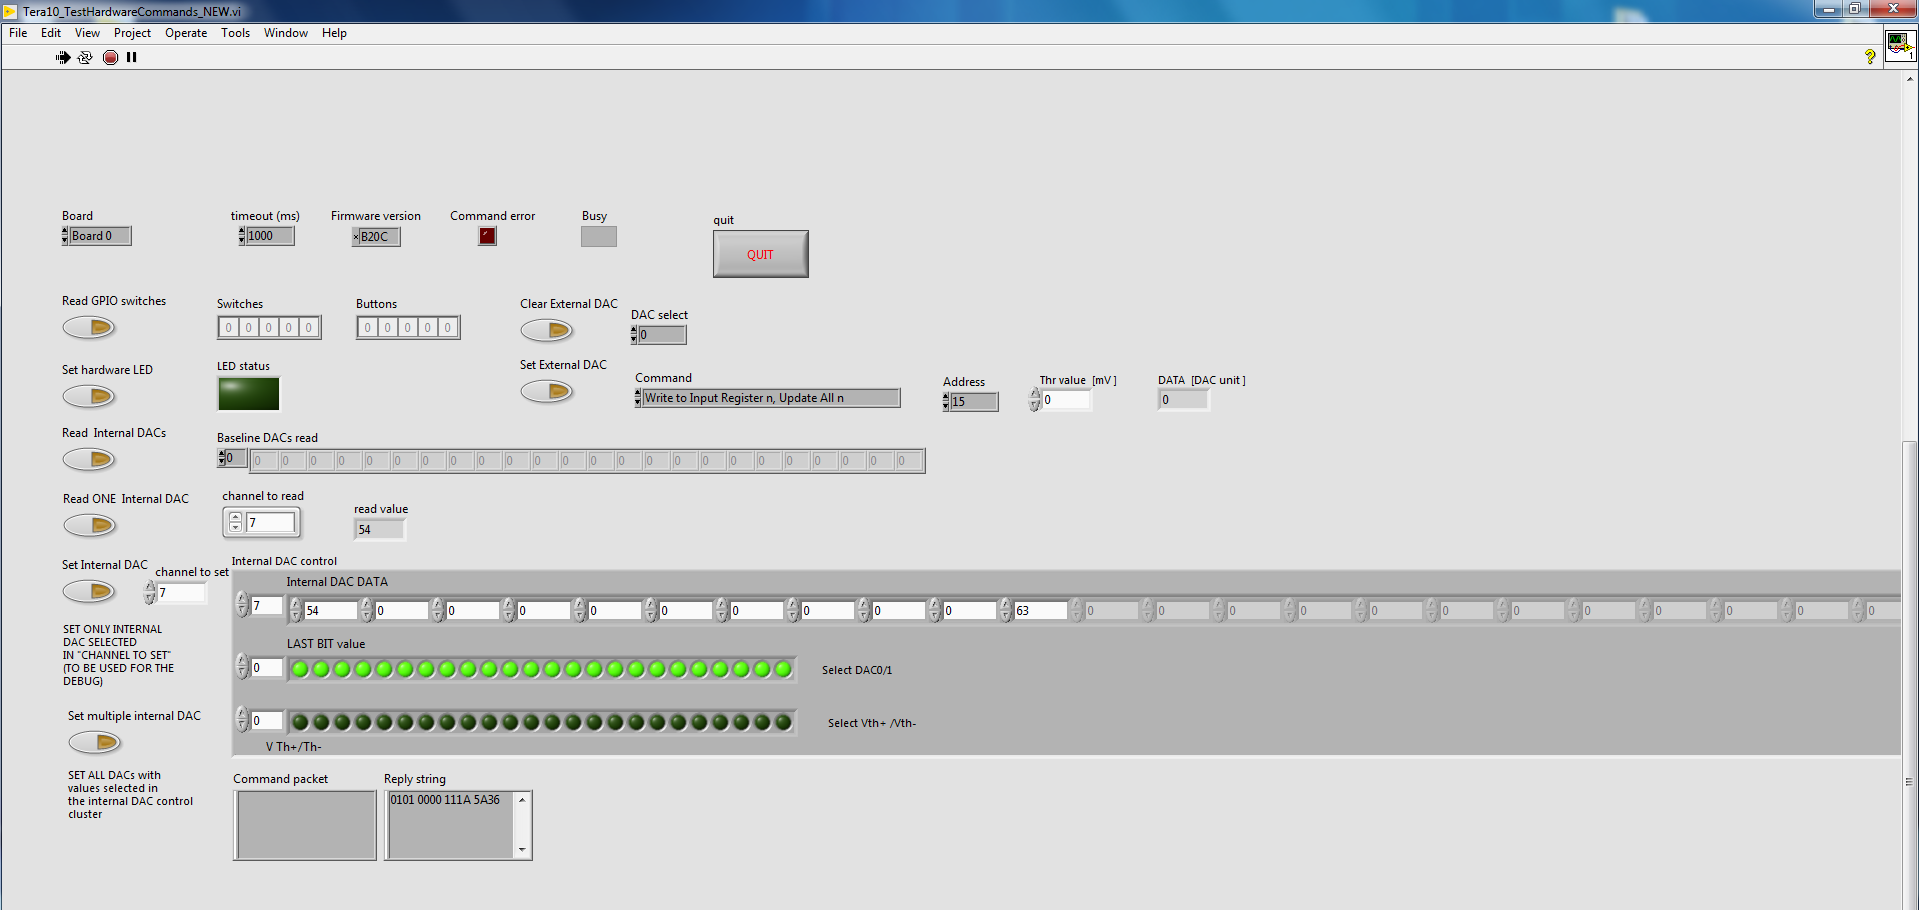
\includegraphics[width=0.9\linewidth]{IMG/ch3/LABVIEW2}
	\caption{LabVIEW Test Hardware Commands program. The white rectangles are inputs, the user can set a value bounded between 0 and 63, the green dots and the buttons are 1 bit inputs, while the more grey squares are outputs}
	\label{fig:labview2}
\end{figure}
\section{Xilinx 7 Series}
\noindent The FPGA used in this project is a Kintex 7, however Xilinx 7 series comprise four FPGA families that address a complete range of system requirements; in figure \ref{fig:kintex72} it can be seen a comparison between the four different families.
\begin{figure}[H]
	\centering
	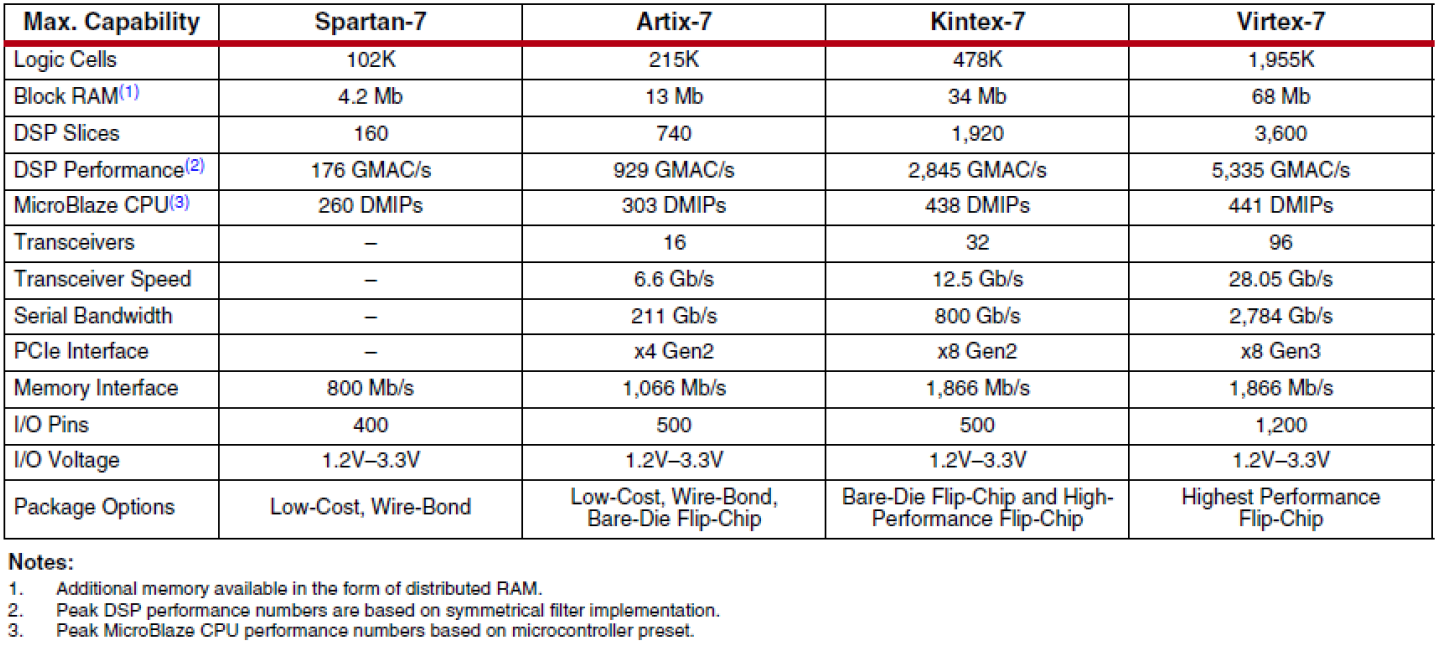
\includegraphics[width=0.9\linewidth]{IMG/ch3/KINTEX72}
	\caption{Comparison between the different boards from the Xilinx 7 line-up}
	\label{fig:kintex72}
\end{figure}
\begin{itemize}
	\item  \textbf{Spartan-7} Family: Optimized for low cost, lowest power, and high
	I/O performance. Available in low-cost, very small form-factor
	packaging for smallest PCB footprint.
	\item \textbf{Artix-7} Family: Optimized for low power applications requiring serial
	transceivers and high DSP and logic throughput. Provides the lowest
	total bill of materials cost for high-throughput, cost-sensitive
	applications.
	\item \textbf{Kintex-7} Family: Optimized for best price-performance with a 2X
	improvement compared to previous generation, enabling a new class
	of FPGAs.
	\item \textbf{Virtex-7} Family: Optimized for highest system performance and
	capacity with a 2X improvement in system performance. Highest
	capability devices enabled by stacked silicon interconnect (SSI)
	technology.
\end{itemize}
\subsection{Kintex 7 kc705}
\noindent In the MoVe\_IT project are used FPGA boards like the one in figure \ref{fig:kintex}, a Xilinx Kintex 7 kc705 development board\cite{kintex7}.
\begin{figure}[H]
	\centering
	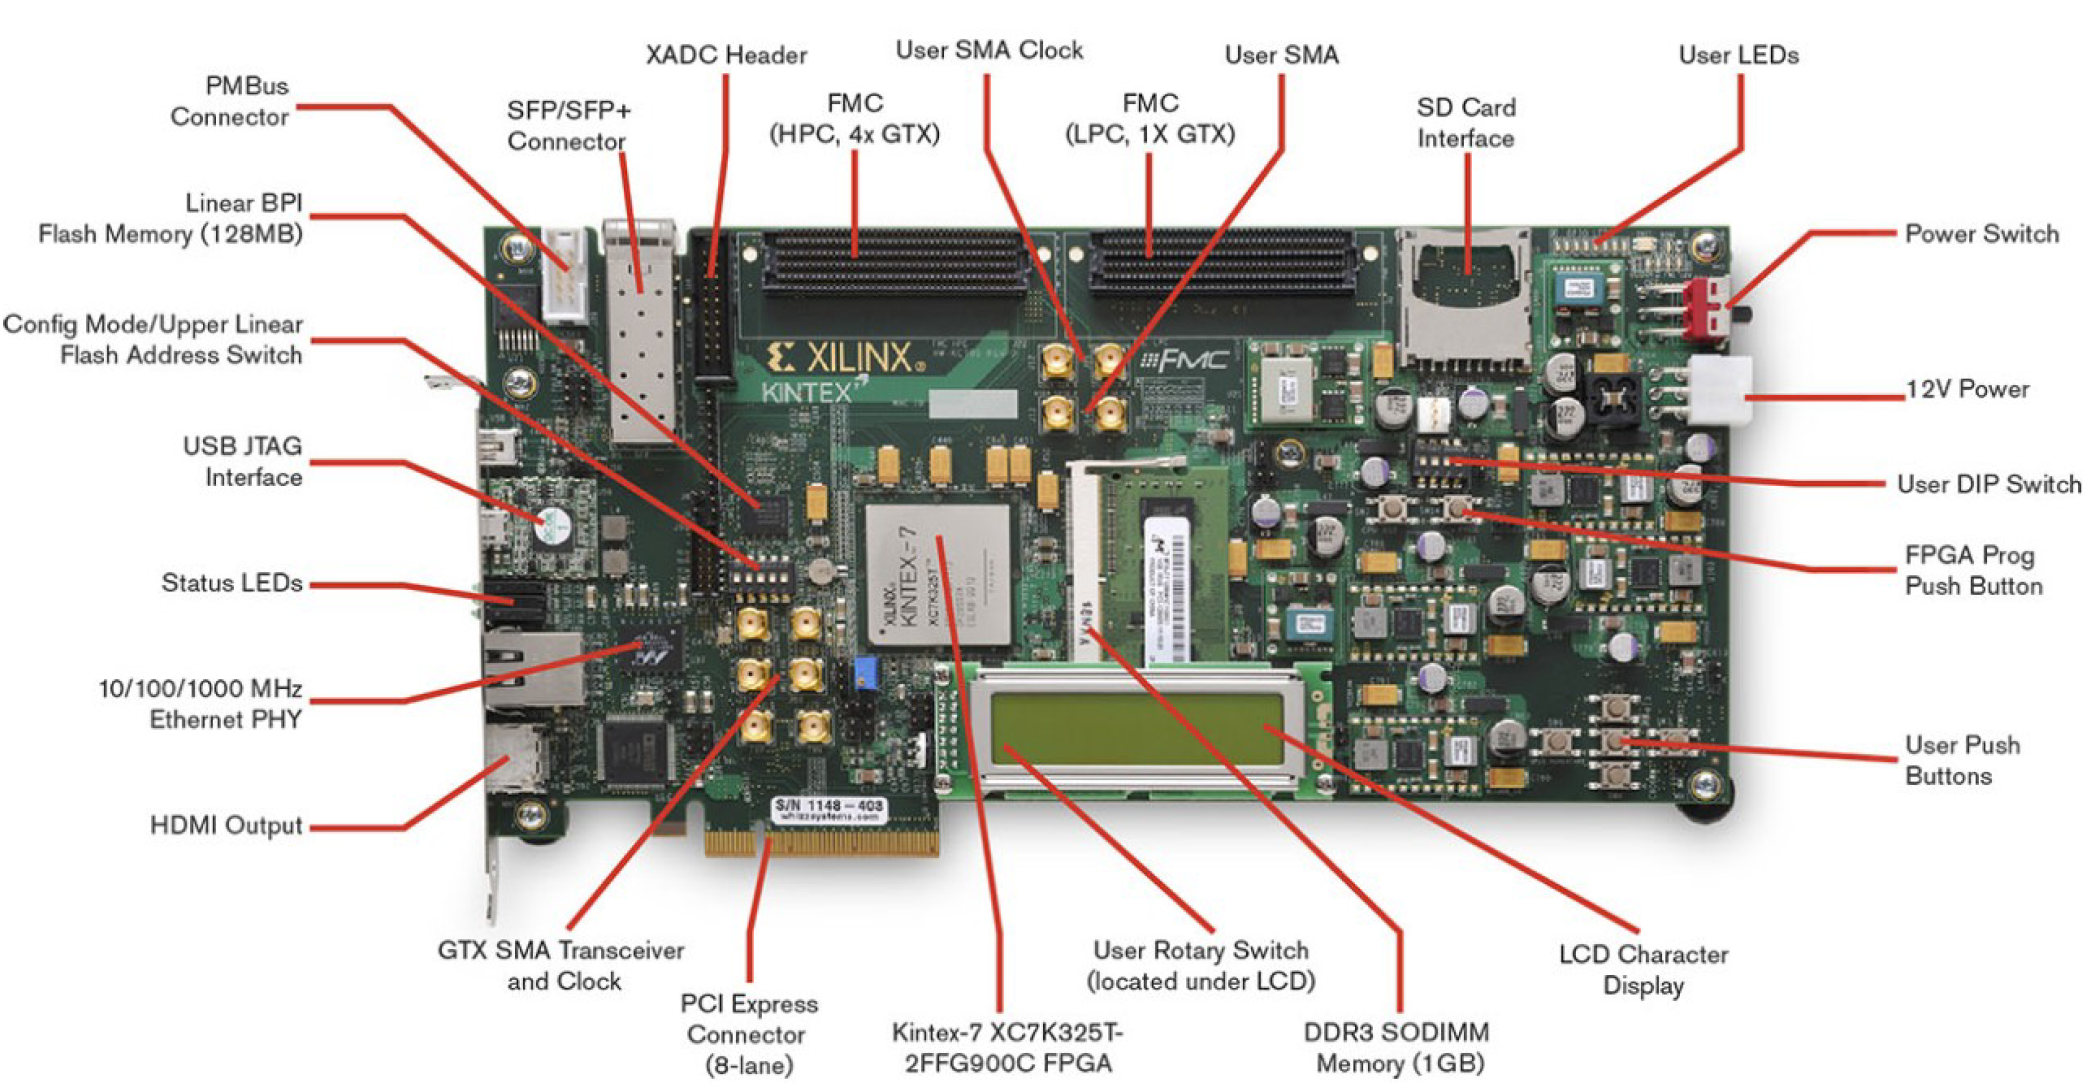
\includegraphics[width=0.9\linewidth]{IMG/ch3/KINTEX}
	\caption{Xilinx Kintex 7 kc705 development board}
	\label{fig:kintex}
\end{figure}
\noindent Its main characteristics are:
\begin{itemize}
	\item \textbf{RJ45 Ethernet Jack}, direction indicator LEDs and \textbf{PHY chip} allow communication between FPGA and PC to speeds up to 1Gb/s.
	 \begin{figure}[H]
	 	\centering
	 	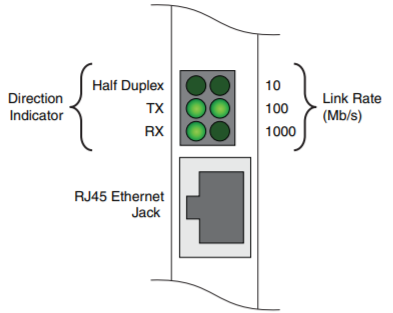
\includegraphics[width=0.2\linewidth]{IMG/ch3/PHY}
	 	\caption{RJ45 connector and status LEDs indicators; the LEDs are disposed in such a way that they are still visible when the board is connected to a PCI Express enclosure.}
	 	\label{fig:phy}
	 \end{figure}
	\item \textbf{Two FMC} (FPGA Mezzanine Connector). One is HPC (High Pin Count) with 400 pins that provides connectivity for up to:
	\begin{itemize}
		\item 160 single-ended or 80 differential user-defined signals;
		\item 159 ground and 15 power connections;
		\item 4 differential clocks;
	\end{itemize}
	\noindent and one is LPC (Low Pin Count) with 160 pins that provides connectivity for up to:
	\begin{itemize}
		\item 68 single-ended or 34 differential user-defined signals;
		\item 61 ground and 10 power connections;
		\item 2 differential clocks;
	\end{itemize}
	For the purpose of this project the two connectors are equal, since they are used only the pins common to both pin configurations.
	\item 16x2 \textbf{LCD Display} used to show information such as: organization name, project name, firmware version and board number.
	\item \textbf{LEDs}, \textbf{buttons} and \textbf{dip switches} are useful tool for debugging purpose. In this case the LEDs and the buttons can be used to verify the correct operation of the FPGA-PC communication while the dip switches are used to configure the board number (operation mandatory when using more than one board at the time).  
	\item The \textbf{FPGA Chip} is the XC7K325T; in figure \ref{fig:kintex7} can be seen the most important parameters.
	\begin{figure}[H]
		\centering
		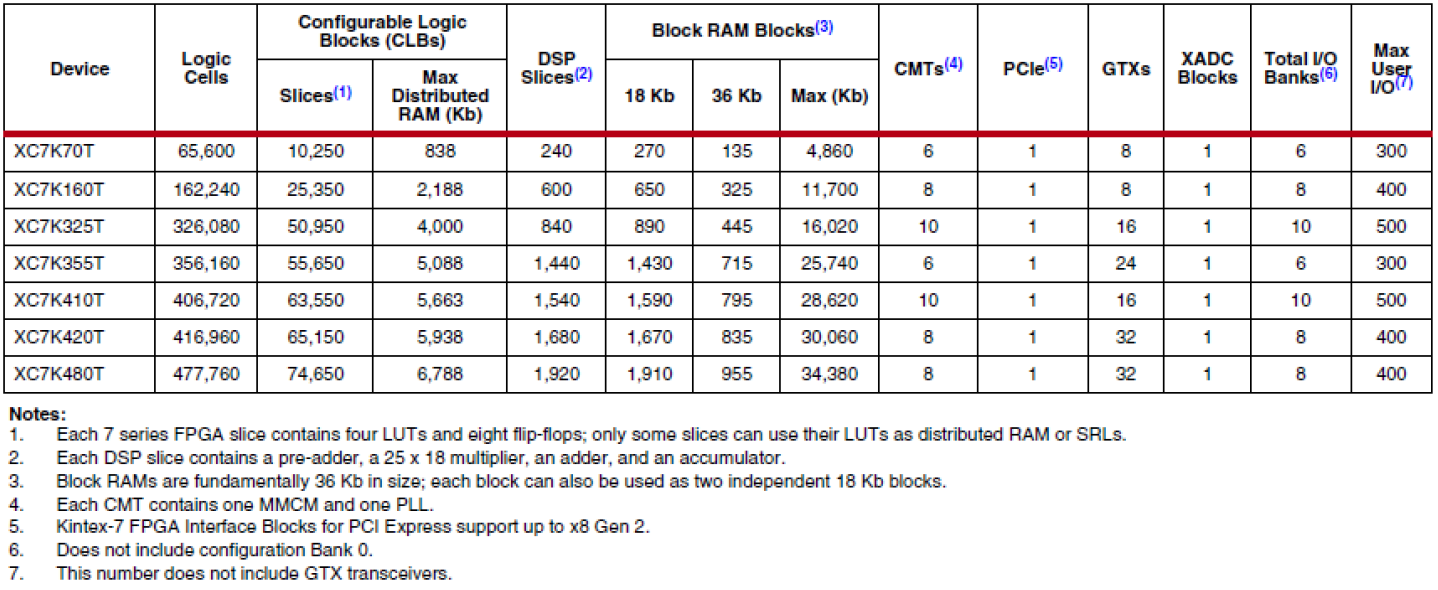
\includegraphics[width=0.9\linewidth]{IMG/ch3/KINTEX7}
		\caption{Xilinx Kintex 7 XC7K325T main parameters; each logic cell is made up with 1 MUX, 1 LUT and 1 Filp Flop; one slice is made up with 4 LUTs, 8 Flip Flop and a Carry Chain; 1 CLB = 2 Slice; DSP = Digital Signal Processing; BRAM = Block RAM}
		\label{fig:kintex7}
	\end{figure}
	\item \textbf{Flash Memory} used to store the firmware binfile wile the card is not powered.
	\item \textbf{USB JTAG} interface used to program the board.
	
\end{itemize}


































